\documentclass[10pt, a4paper]{article}
\usepackage{geometry}
\usepackage[english]{babel}
\usepackage[utf8]{inputenc}
\usepackage{amsmath}
\usepackage{csquotes}% Recommended
\usepackage{graphicx}
\usepackage{caption}
\usepackage[sort&compress, numbers, square]{natbib}
\usepackage{caption}
\usepackage{subcaption}
\usepackage{parskip}
\usepackage{palatino}
\usepackage[compact]{titlesec}
\titlespacing{\section}{0.3pt}{*0}{*0}
\titlespacing{\subsection}{0pt}{*0}{*0}
\titlespacing{\subsubsection}{0pt}{*0}{*0}

\setlength{\parindent}{15pt}
\setlength{\parskip}{0.25cm plus0mm minus0mm}

\newgeometry{margin=2.5 cm}


\begin{document}
\section*{Personnel}
\begin{enumerate} 
\item PI Craig McClain (Assistant Director of Science, Duke University, National Evolutionary Synthesis Center) will oversee students, data collection, database development and management, as well as provide leadership for the project.
\item PI Josef Uyeda (Postdoctoral Fellow, University of Idaho) will oversee students, method development and analyses.
\end{enumerate}
\clearpage
\section*{Framework and Objectives}
Life requires energy, and the transformation and flow of energy link all levels of biological organization \cite{McClain2012}. Although energy is a key currency across biological systems, we still have little idea of how energy usage has changed as species have evolved. The amount of energy allocated to different organismal functions affects allometric scaling, how physiological, ecological, and life history relationships scale with body size \cite{Peters1983, Calder1984}. Finite resources, trade-offs and genetic constraints force organisms to employ alternative strategies to reproduce and maintain organismal functioning \cite{McClain2014}. Therefore, changes in allometries can reflect evolutionary change in the energy budgets and life-history strategies of species. While previous research has applied phylogenetic comparative methods to document differences in allometries for predefined clades, we lack the necessary tools to directly study the evolution of allometry across phylogenies and distinguish the ecological drivers of these changes. This is because evolutionary allometries require cross-species data to estimate, yet the underlying energetic scaling relationships themselves evolve among lineages according to processes that may not follow arbitrary taxonomic boundaries.  \

\textbf{To fully understand the processes governing the evolutionary dynamics of energy usage across the tree of life, we will develop and implement a truly tree-based approach.  We propose to use a phylogenetic comparative approach to uncover the long-term macroevolutionary dynamics of energy usage among vertebrate clades, as revealed by allometric scaling relationships. Specifically, we will utilize phylogenetic relationships to uncover the evolutionary history of metabolic scaling with size along with other prominent energetic scaling relationships (e.g. longevity, growth rate, home range). We will develop novel Bayesian comparative regression tools to study the evolution of these allometric scaling relationships.}
\section*{Background}
Typical allometric scaling relationships take the form of 
\[B = b_0M^a\]
B is dependent variable of interest, e.g. metabolism (as in the case here), growth, lifespan, home range. bo is an intercept term that and may or may not vary among clades and with different ecologies.  M is body mass of the organism. a is the scaling exponent of the relationship. \

The most prominent of the allometric scaling equations relate metabolic rate and body size, known as the “mouse-to-elephant” curve in mammals.  This relationship has been observed since the early twentieth century \cite{Benedict1938} but continues to inspire debate of possible causes underlying the relationship (e.g. \cite{West1999a, West1999b, Bokma2004}). Despite nearly a century of work, there is no consensus on several fundamental aspects of metabolic scaling. Controversy remains as to the value of the slope between metabolic rate and body size (often debated to equal either $\frac{2}{3}$ or $\frac{3}{4}$) (\cite{West1997, West1999a, West1999b, Brown2004, Savage2004, FarrellGray2005, IsaacCarbone2010, WhiteSeymour2003, Hudson2013, Dodds2001}; reviewed by \cite{Bokma2004, IsaacCarbone2010}) and the processes that actually determine these scaling exponents \cite{West1999a, West1999b, Banavar2002, Brown2004, CyrWalker2004, Glazier2005, Kolokotrones2010, Apol2008, Banavar2010, Maino2013}. \

In addition, a lack of consensus also surrounds whether metabolism has universal scaling exponents or differs among clades  \cite{HayssenLacy1985, McKechnieWolf2004, Glazier2005, McKechnie2006, White2006, Makarieva2008, Sieg2009, Capellini2010, DeLong2010}. For example, basal metabolic rates are often shown to be higher in passerine birds compared to nonpasserines; however, this difference disappears when phylogenetic independent contrasts are used (reviewed in \cite{McKechnieWolf2004}). Shrews, cetaceans, and pinnipeds have metabolic rates exceeding other mammals \cite{Bartels1982, Andersen1969}. Slopes and intercepts of the scaling relationships may differ between placental mammals and marsupials \cite{McNab1988, AgutterWheatley2004}.  Differences also occur across diet types in mammals \cite{McNab1988} and anurans \cite{SantosCannatella2011} but may largely reflect clade differences as well \cite{ElgarHarvey1987}.  \

\textbf{Despite the lack of consensus, these potential clade differences suggest that fundamental shifts may have occurred in the evolution of metabolism.} Clade differences also exist in other allometric scaling relationships (e.g., home range size \cite{Tucker2014}). Prior research into these relationships has largely concentrated on contemporary patterns and lacked a deeper time, i.e. phylogenetic, perspective. These studies have used phylogenies in a PGLS framework to simply account for nonindependence of shared evolutionary histories (e.g. \cite{Sieg2009, Capellini2010}). No study has used a phylogenetic approach using biologically-realistic models of adaptation to specifically reveal the evolutionary dynamics of allometric scaling and uncover the potentially rich macroevolution of energy usage. This reflects a lack of methods in a comparative framework that can use across-species data to estimate shifts in allometric scaling.  \

Our preliminary work has already yielded exciting findings. We synthesized a phylogenetic tree from existing vertebrate timetrees and a dataset of 855 published standard metabolic rates (SMR). We find evidence of evolutionary shifts in both intercept and slope in the allometric scaling relationship between body mass and SMR (Figure 1). We have developed a method that not only detects well-known shifts in the intercept associated with endothermy, but also shifts in both slope and intercept in several smaller, but well-defined clades such as snakes and lungless salamanders (Figure 1). Ours is the first method that does not assign groups a priori. Instead, we extend our previous software \cite{UyedaHarmon2014} to detect and identify the clades for which shifts have occurred directly from the phylogenetic comparative data. We also include additional predictors in our regression framework, and have extended previous results by identifying significant curvature in the relationship between SMR and body mass across all major vertebrate groups \cite{Kolokotrones2010}. We show that this result appears general across vertebrate taxa, and not simply a reflection of lineage-specific shifts in clades with extreme body sizes. This ability to include a range of predictors in a regression framework enables us to ask what factors influence shifts in the slope and intercept of allometric scaling relationships, opening up new avenues for inquiry into the evolution of energetics.
\section*{Research Aims}
Here we seek to examine the evolution of a set of fundamental relationships, i.e. allometric relationships, in biology.  Specifically, we build on prior macroecological approaches by applying a macroevolutionary lens to elucidate the evolution of energy usage. Our specific research aims are to address three major questions, each of which will require the development of novel analytical tools.
\begin{enumerate}
\item When and in what clades did major shifts in metabolic scaling and other energetic relationships occur? Alternatively, is scaling evolutionary conserved, suggesting a universal first principle driver for energy scaling relationships?
\begin{itemize}
\item To answer this question, we will develop novel Bayesian phylogenetic comparative methods for inferring shifts in allometric scaling relationships that maximally uses available data and reflects realistic evolutionary processes.
\end{itemize}
\item How do allometric scaling relationships vary with environmental variables? Do predictable relationships emerge between environment, life history, and transitions between  $\frac{2}{3}$ or $\frac{3}{4}$ scaling?
\begin{itemize}
\item We will develop and implement an Bayesian phylogenetic regression framework that we will use to test for the effects of life history traits and environment on allometric scaling parameters. 
	\end{itemize}
\item Do rates and magnitudes of shifts in scaling relationships vary over time and geologic ages, and what are the predictors of these changes?
	\begin{itemize}
\item We will implement hierarchical models that allow estimation of the rate and magnitude of shifts in evolutionary allometry, and test whether changes in rate are driven by climatic shifts.
	\end{itemize}
\end{enumerate}

These aims will address novel questions regarding the dynamics of evolution in energy budgets of organisms at macroevolutionary scales, while simultaneously providing powerful, general methods and software for applying the phylogenetic comparative method to studying adaptation and evolution. For example, understanding allometric and correlative relationships, such as clutch size and latitude, are fundamental aspect of macroecology. The development of these methods will allow us to examine how the parameters of these relationships evolved through time.
\section*{Research Approach}
\begin{figure}
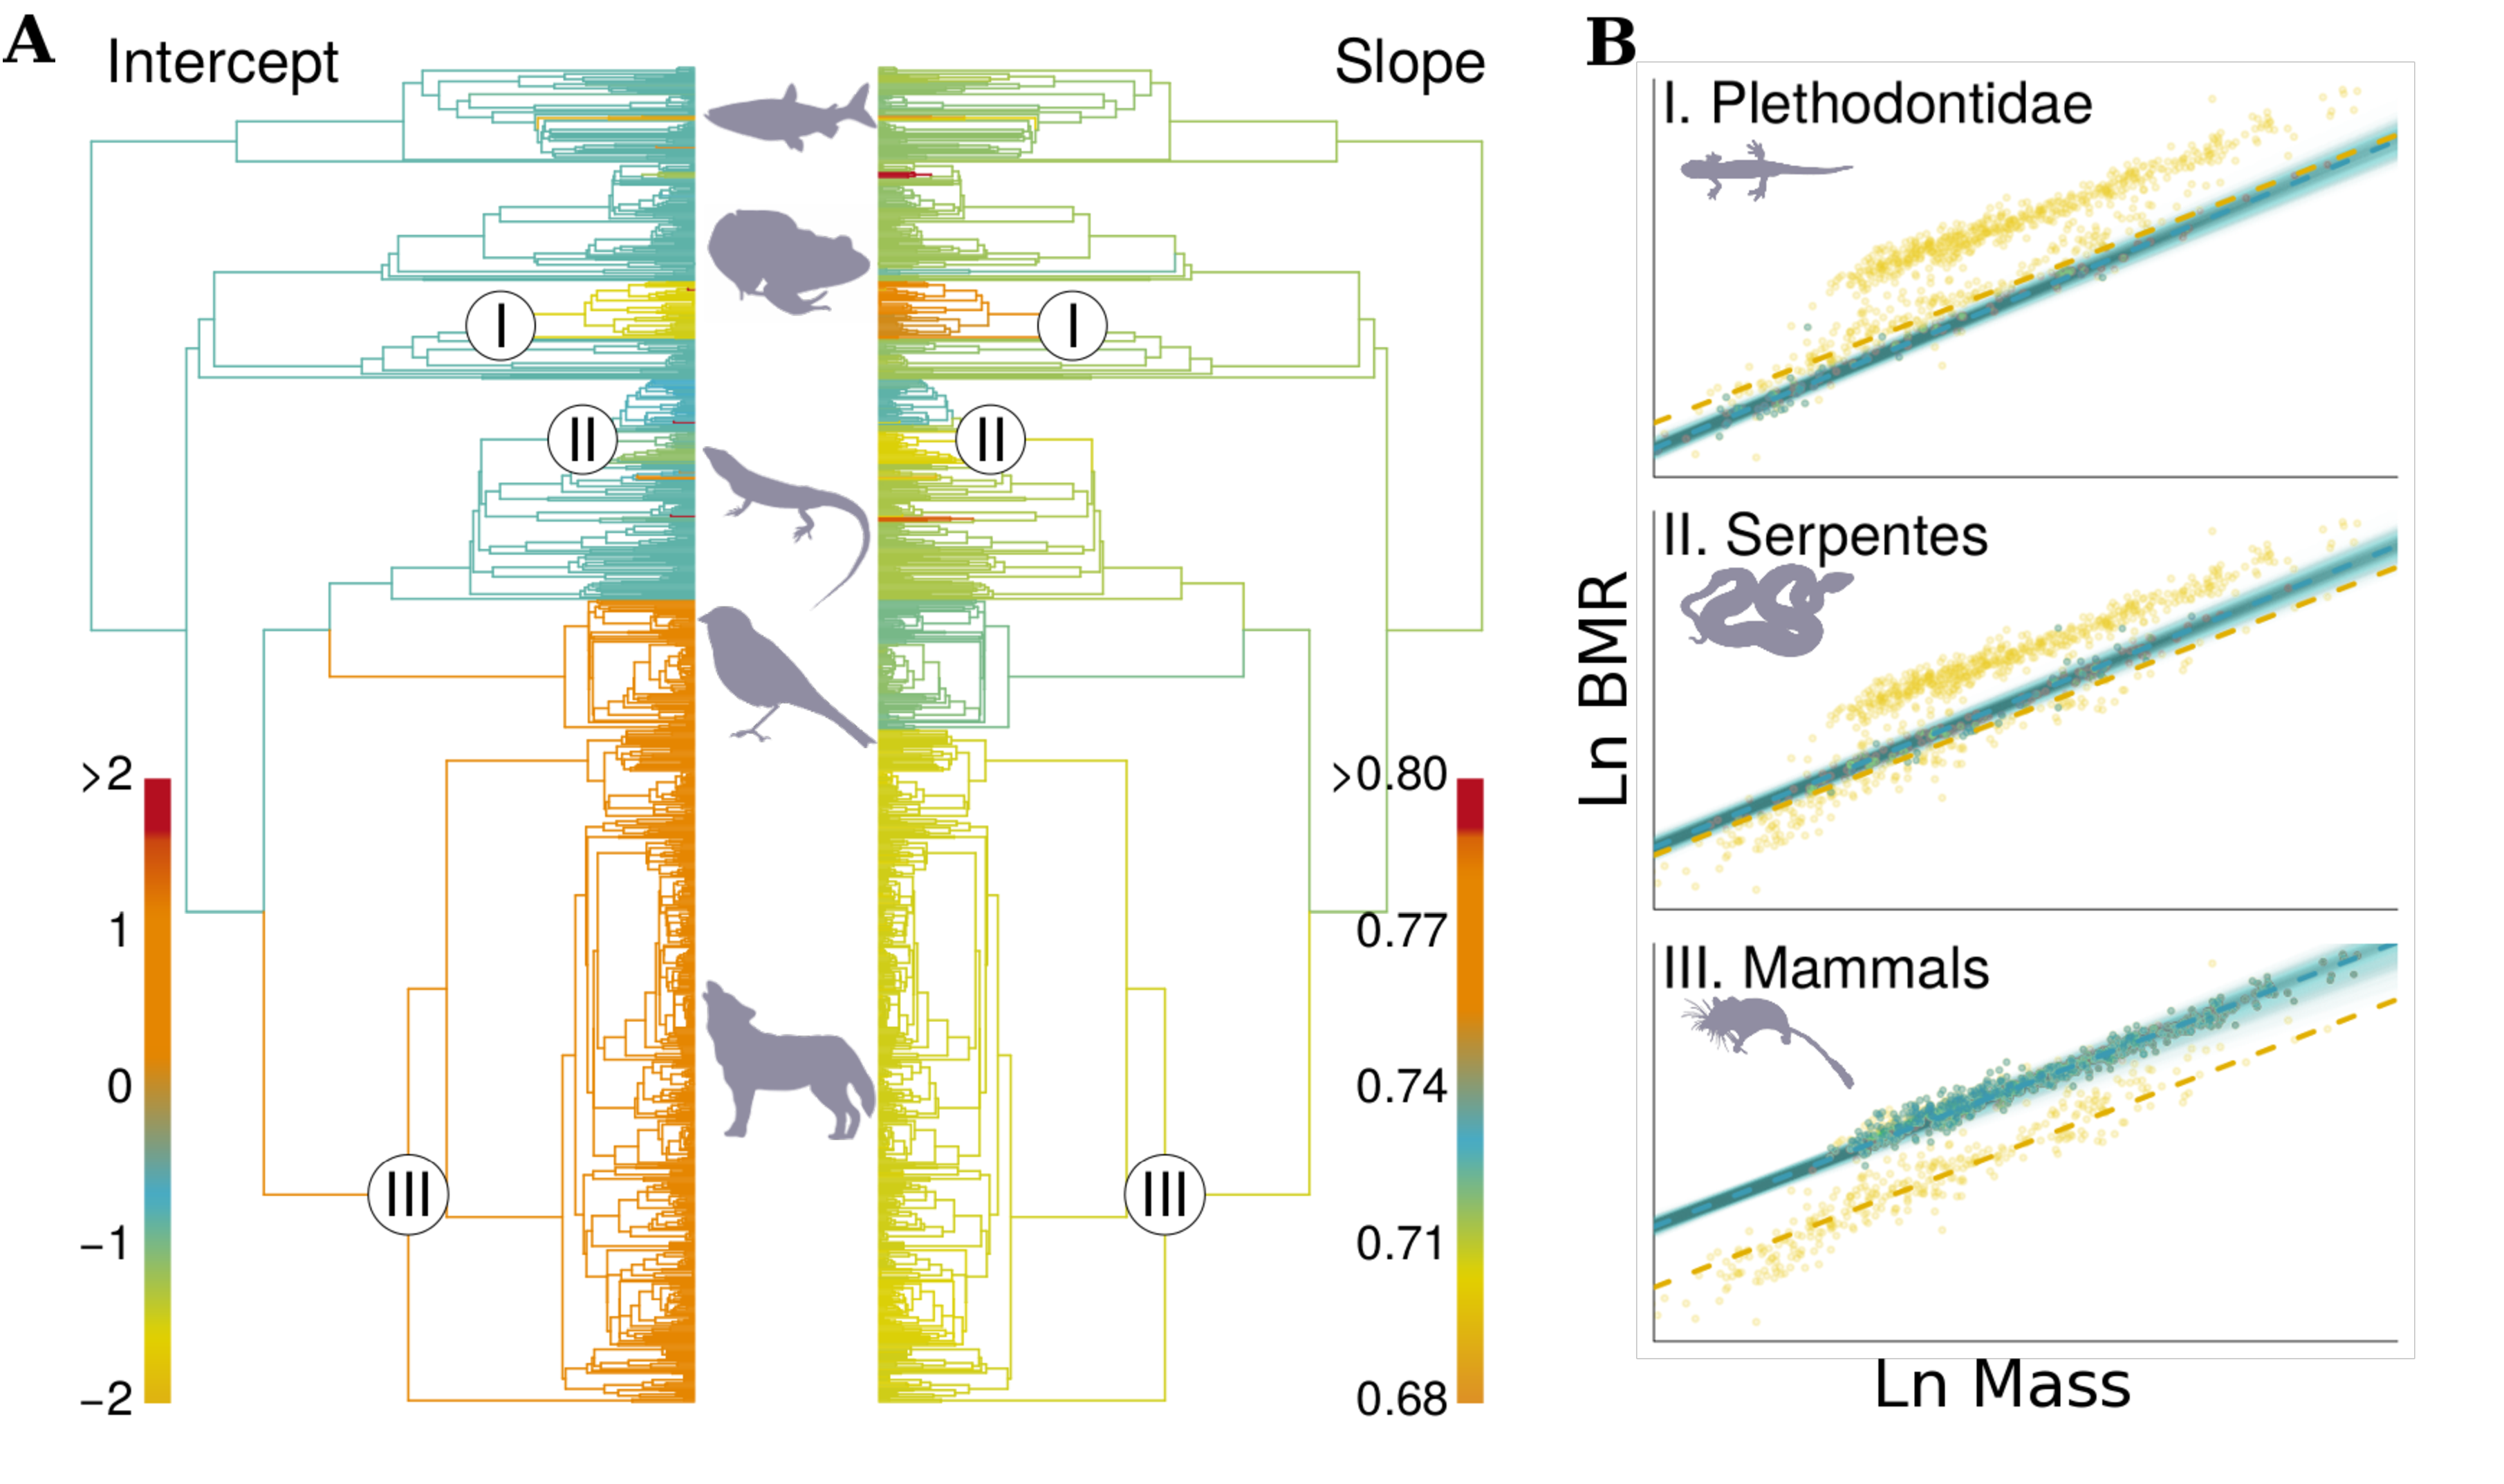
\includegraphics[width=0.95\linewidth]{Figure1} 
\caption{(A) Phylogenies showing the posterior mean intercept and slope for the allometric regression between metabolic rate and body mass across the vertebrate phylogeny as identified by \textit{bayou}. (B) Allometric relationships for clades identified as having a high posterior probability of a shift in the same analysis (clades correspond to the circled nodes in A). The posterior distribution of the estimated allometry for each clade (in purple) is compared to the inferred ancestral allometry (gold dotted line). }
\label{fig:test}
\end{figure}	

To address our specific aims, we will develop Bayesian phylogenetic comparative models building on our existing software package \textit{bayou} \cite{UyedaHarmon2014}. Specifically, \textit{bayou} uses reversible-jump Markov chain Monte Carlo (MCMC) to search across model-space for shifts in adaptive optima on phylogenetic trees \cite{Green1995, HoAne2014}. The model realistically reflects the biological process of adaptive evolution by using an Ornstein-Uhlenbeck (OU) model to describe trait evolution along the phylogeny \cite{Hansen1997}. Previously, \textit{bayou} could only model fixed optima (as in \cite{ButlerKing2004}). However, we have extended this method to allow for additional predictors, enabling researchers for the first time to leverage reversible-jump model selection to identify  evolutionary dynamics in allometric scaling (Figure 1). \

Our preliminary work has focused on applying this model to a large dataset of SMR values from across the vertebrate tree of life \cite{White2006}. We combined published phylogenies of major vertebrate groups \cite{BinindaEmonds2007, PyronWiens2011, Jetz2012, Pyron2013, Rabosky2013} to build a synthetic phylogeny of vertebrates. We will expand this phylogeny and dataset by building a pipeline for synthesizing published phylogenies obtained from the Open Tree of Life AVAToL project \cite{Cranston2014}. Using OpenTree’s database of study trees, its synthetic topology, and existing tools for synthesizing phylogenetic data (e.g., \cite{Eastman2013}), our pipeline will automatically build a dated, synthetic tree for our study taxa using available timetree calibrations in the database. Our pipeline will provide a powerful tool for generating trees for comparative analyses, as our fully reproducible workflow can be repeated as increasing data and resolution are added to the OpenTree database. In addition to SMR, we will also examine allometries of additional ecological and life history traits (e.g. lifespan, clutch size/offspring number, age at maturity, home range size, population growth) from several databases including:  PanTHERIA for mammals \cite{Jones2009}, FishBase for fish \cite{Froese2000}, and Encyclopedia of Life for birds, amphibians, and reptiles \cite{Parr2014}. Quantification of these additional allometric relationships will allow us to look for concordant shifts and tradeoffs among traits on the phylogeny. We will implement Bayesian data imputation methods to maximally account for incomplete data, enabling full-scale analyses that account for uncertainty while simultaneously maximizing power to estimate the evolutionary process \cite{Rubin1987, NakagawaFreckleton2008, NakagawaFreckleton2011}. Since our method automatically accounts for evolving allometric relationships, we will be able to incorporate the entire phylogeny of vertebrates in a single analysis to study the evolution of metabolic scaling at an unprecedented scale---obtaining for the first time direct estimates of the timing and magnitude of allometric shifts while increasing the accuracy of scaling estimates. This will allow us to determine between $\frac{2}{3}$ or $\frac{3}{4}$ scaling relationships and possible evolutionary transitions between the two---addressing a long-standing debate in macroecology.  \

For research question two, we will seek to identify the extrinsic predictors (e.g.,  environmental, ecological and life history traits) of variation in allometric scaling.  \textit{While previous methods have used a phylogenetic comparative approach to studying allometric scaling in metabolism, they do not account for the process of adaptation} \cite{HansenOrzack2005, HansenBartoszek2012}. Specifically, the models employed are only appropriate for testing intrinsic effects that directly shift metabolic rate (e.g. the instantaneous increase of mass with linear dimensions). Questions regarding extrinsic effects, or intrinsic traits that do not have a direct link to metabolism (e.g. sexual dimorphism, parental investment etc.) are therefore outside the scope of the most commonly applied methods (i.e. PGLS). This is because the models only account for the current state of the predictor variable, rather than accounting for the adaptive lag that occurs given a long-history of imperfect adaptation to variable conditions. This widely unappreciated fact not only results in biased estimates and ignores the process of adaptation, but ignores the fact that this lag itself is of evolutionary interest, as recent selective history for metabolic traits can have important consequences for organisms and disease susceptibility \cite{Wisloff2005}. To address these concerns, Hansen and colleagues \cite{Hansen2008} developed a powerful stochastic linear modeling regression framework using OU models. However, the approach of Hansen et al. \cite{Hansen2008} is a likelihood-based implementation that does not allow the scaling relationship itself to evolve. By uniting this approach with bayou, we will be able to ask new questions such as whether observed shifts in allometric scaling can be explained by hypothesized effects such as diet or trophic level \cite{McNab2000}, parental investment \cite{Koteja2000}, or environmental temperature \cite{Gillooly2001}. We will apply our methods to uncover the ecological correlates that favor transitions in allometric scaling.\

To address research question three, we will build hierarchical Bayesian models that infer parameters controlling the rate and magnitude of shifts in allometric scaling \cite{Gelman2003}. We will test whether shifts in allometric scaling relationships have occurred with greater frequency across geologic periods or eras---associated with major changes in the environment of earth. Additionally, we will test for an association between the rate of shifts in scaling and global climate timeseries, such as temperature and oxygen availability (compiled at the global level by Payne \cite{Payne2013}). These tests will address whether shifts in allometry and energy budgets can be explained by changes in global climate, making a wide-range of hypotheses testable for which no trait data is available in the fossil record. For example, by placing a hyperprior on the rate of shifts in slope and intercept that is dependent on global temperature, we will obtain estimates of whether or not shifts in energetic scaling are associated with particular climate conditions, or whether dramatic changes in climate trigger global shifts and diversification in the energy budgets of organisms. One specific prediction would be that as increased temperatures, \textit{ceteris paribus}, increase energy requirements for basic maintenance \cite{Gillooly2001}, i.e. metabolism, this would reduce energy available for reproduction and trigger shifts in life history strategies \cite{Kearney2012}.\

Our approach differs from previous methods by simultaneously allowing us to 1) identify shifts in across species scaling relationships without predefining clades 2) realistically account for the process of adaptation in a Bayesian framework and 3) identify both intrinsic and extrinsic factors influencing scaling relationships \cite{HansenBartoszek2012, UyedaHarmon2014, HoAne2014}. By doing so, we will elucidate the macroevolutionary drivers of change in energetic relationships and open new avenues of research in macroevolution and macroecology. Furthermore, our methods and software will provide a powerful, flexible and extensible framework for modeling adaptive evolution on phylogenies that will have broad applicability to a wide-range of empirical questions.
\section*{Broader Impacts}
Our public outreach component focuses on curriculum development.  Our target audience will be pr-college and college courses with the goal of introducing evolutionary concepts and having students engage in inquiry based activities with real data sets. This goal aligns with both the Vision and Change report that guides college level biology education reform, and the Next Generation Science Standards (NGSS).  The Vision and Change Report identifies “Pathways and transformations of energy and matter” and “Evolution” as two of the five core biological concepts, and includes the ability to use quantitative reasoning and to apply the process of science as two disciplinary practice skills.  The NGSS include components in Life Science for middle and high school that focus on evolution (Biological Evolution:Unity and Diversity).  Moreover, the eight practices of science and engineering that the NGSS Framework identifies as essential for all students include: 4. Analyzing and interpreting data and 5. Using mathematics and computational thinking.  We will work specifically with BioQUEST and the QUBES project (a collaboration is initiated) to develop curriculum materials and disseminate these to classrooms.  Tree thinking is a key component in understanding evolutionary processes, and scientific processes such as inference, visualization, modeling and communication.  However, tree thinking is an extremely challenging skill to develop.  This curriculum will provide an entry point to explore tree thinking in the context of allometry, supporting the development of several key skills and understanding of evolution.  The synthesized allometric data and phylogenies created for this project will provide the key data necessary for this materials.  We will design curricula and activities using web-based software to allow students to explore trait evolution across the tree of life. By connecting our software to OpenTree API’s, students will be able to custom select phylogenies and trait data for taxa of interest and dynamically visualize the evolution of these traits. 
\clearpage

\renewcommand{\thepage}{}
\bibliographystyle{cj}
\bibliography{metabolism.bib}


\end{document}